\subsection{Simulación de control}

Cada articulación se verificó de forma individual con el modelo
\texttt{motor\_2gdl\_ctrl.slx}. La tabla~\ref{tab:ctrl} resume el seguimiento de
la trayectoria de P7 con carga mecánica y la figura~\ref{fig:esc} muestra la
respuesta al escalón de 30$^\circ$.

\begin{table}[H]
    \centering
    \caption{Seguimiento de la trayectoria de P7 por articulación ($T_s=10$~ms, carga incluida).}
    \label{tab:ctrl}
    \small
    \begin{tabular}{lccccc}
        \toprule
        Articulación & RMS P [$^\circ$] & RMS P+FF [$^\circ$] &
        Máx P+FF [$^\circ$] & $|V|_{max}$ [V] & $|i|_{max}$ [A] \\
        \midrule
        Joint1 & 0,168 & 0,094 & 0,252 & 0,515 & 0,033 \\
        Joint2 & 0,234 & 0,091 & 0,263 & 0,531 & 0,034 \\
        \bottomrule
    \end{tabular}
\end{table}

El escalón de 30$^\circ$ presentó un sobreimpulso de 0,18\% en Joint1 y 0\% en
Joint2, con tiempos de establecimiento de 111 y 110~ms y errores finales de
0,22$^\circ$ y 0,20$^\circ$. La prealimentación redujo el error RMS entre 44\% y
61\%. La robustez ante variaciones de $J$ entre $0{,}5J$ y $2J$ mantuvo el
sobreimpulso por debajo de 2,2\%.

\begin{figure}[H]
    \centering
    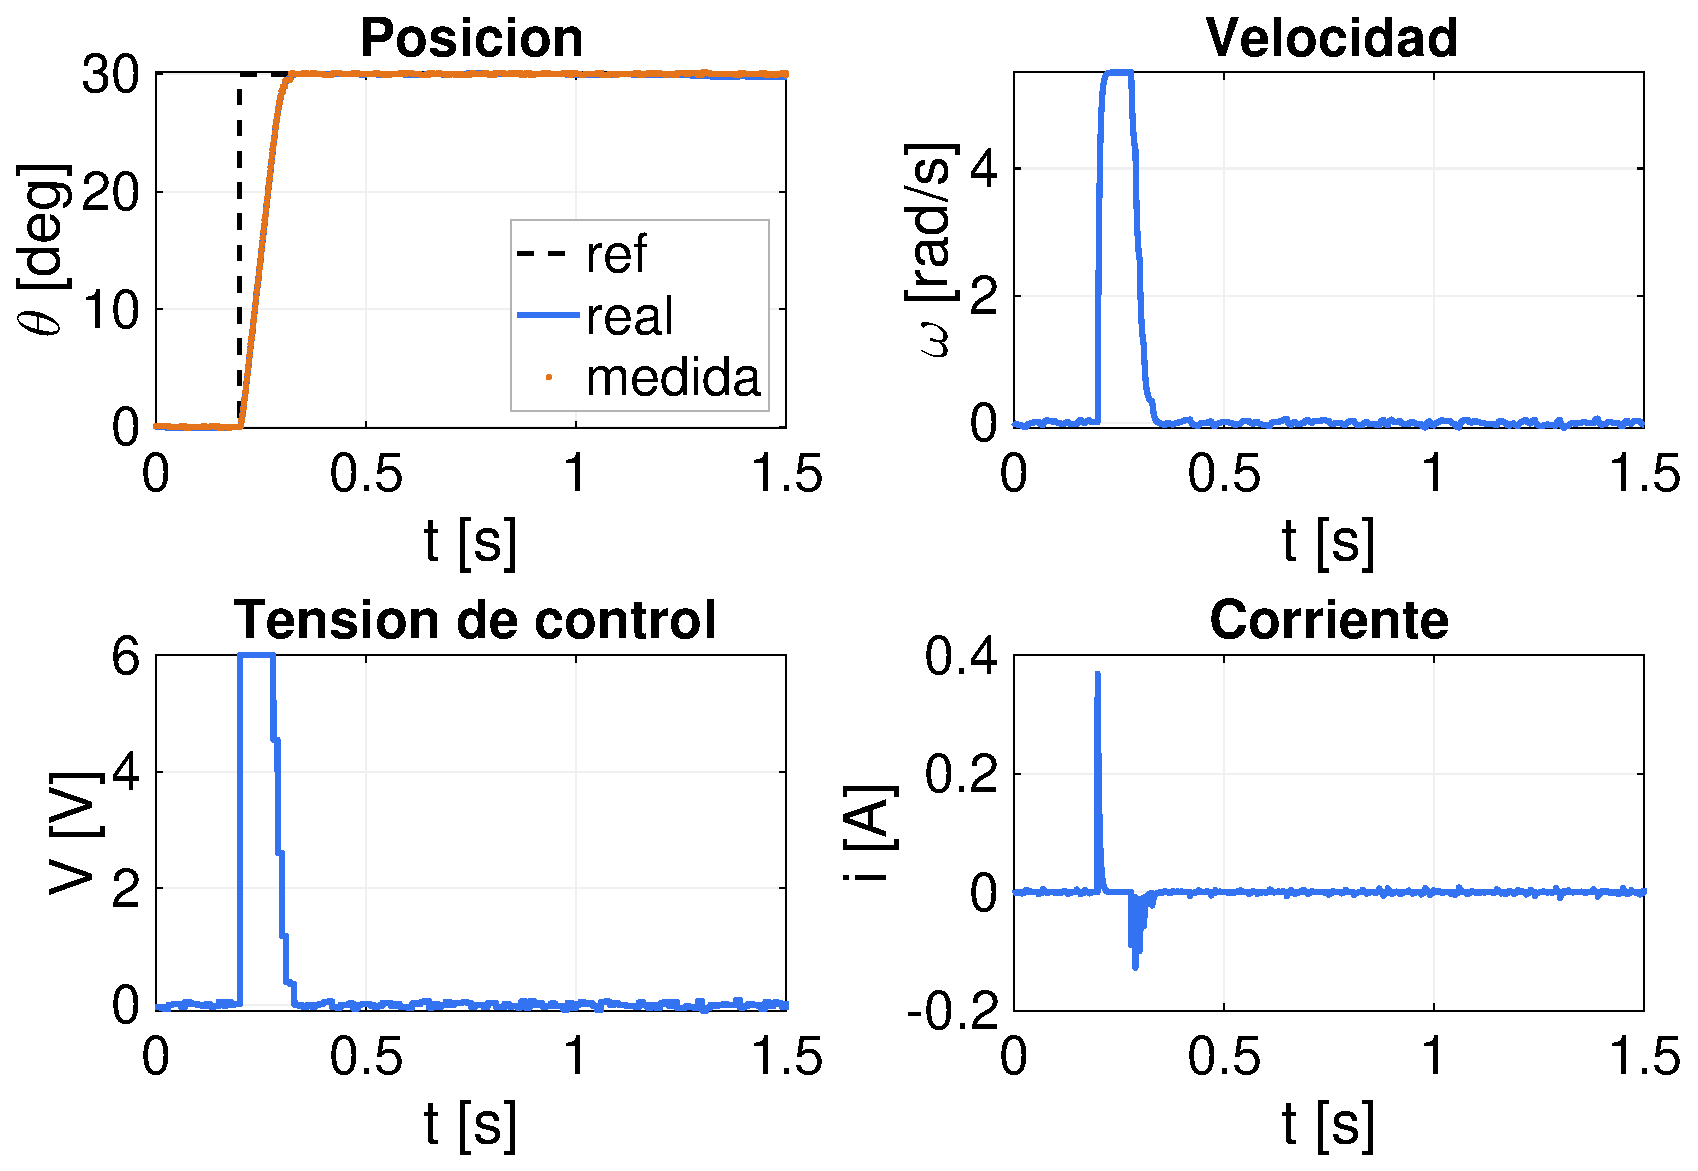
\includegraphics[width=0.62\linewidth]{figuras/control_escalon.eps}
    \caption{Respuesta al escalón de 30$^\circ$ en Joint1.}
    \label{fig:esc}
\end{figure}
